
\documentclass[14pt]{beamer}

\usepackage{color}
\usepackage{tikz}
\usepackage{graphicx}

\usetheme{Warsaw}
\begin{document}

\title{Simulation of a particle detector}
\author{Arnaud Schils \\ Simon Lardinois}
\maketitle

\begin{frame}
\frametitle{Summary}

\begin{enumerate}
  \setlength\itemsep{1.4em}
  \item Particle detector physics
  \item Computing the \textcolor{red}{potential} in the detector
  \item Computing the \textcolor{red}{current} induced by a particle
  \item Conclusion
\end{enumerate}
\end{frame}

\begin{frame}

\frametitle{Particle detector physics}
\framesubtitle{The detector}

%\textcolor{red}{strips}: cathode

\begin{figure}[H]
\begin{center}
	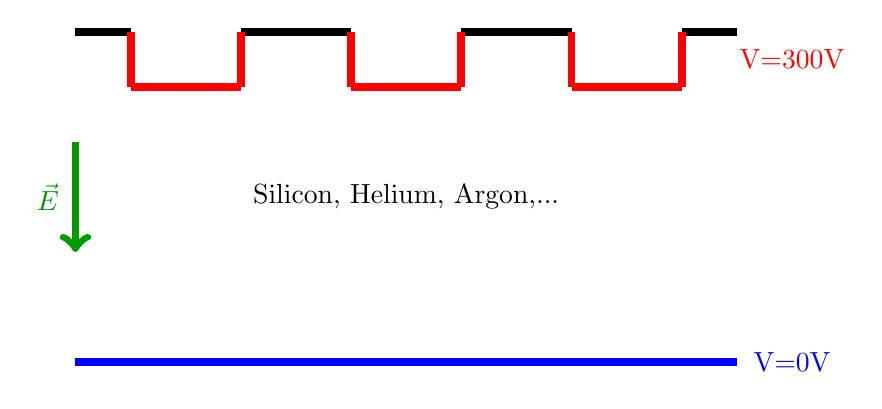
\begin{tikzpicture}[scale=0.7]
    \draw[line width=1mm, black] (-6,3) -- (-5,3);
    \draw[line width=1mm, black] (-3,3) -- (-1,3);
    \draw[line width=1mm, black] (1,3) -- (3,3);
    \draw[line width=1mm, black] (5,3) -- (6,3);

    \draw[line width=1mm, red] (-5,2) -- (-3,2);
    \draw[line width=1mm, red] (-1,2) -- (1,2);
    \draw[line width=1mm, red] (3,2) -- (5,2);

    \draw[line width=1mm, red] (-5,3) -- (-5,2);
    \draw[line width=1mm, red] (-3,3) -- (-3,2);

    \draw[line width=1mm, red] (-1,3) -- (-1,2);
    \draw[line width=1mm, red] (1,3) -- (1,2);

    \draw[line width=1mm, red] (3,3) -- (3,2);
    \draw[line width=1mm, red] (5,3) -- (5,2);

    \draw[line width=1mm, blue] (-6,-3) -- (6,-3);
    \node[blue] at (7,-3) {V=0V};
    \node[red] at (7,2.5) {V=300V};
    \node at (0,0) {Silicon, Helium, Argon,...};

    \node[black!40!green] at (-6.5,0) {$\vec{\text{E}}$};
    \draw[line width=1mm, black!40!green, ->] (-6, 1) -- (-6,-1);


	\end{tikzpicture}
\end{center}
\end{figure}

\end{frame}

\begin{frame}
  \frametitle{Particle detector physics}
  \framesubtitle{Media ionization (I)}


  \begin{figure}[H]
  \begin{center}
  	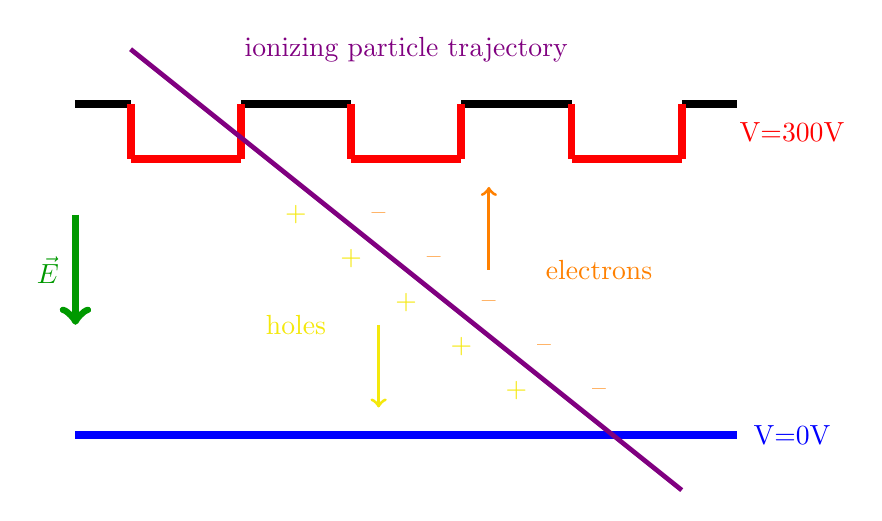
\begin{tikzpicture}[scale=0.7]
      \draw[line width=1mm, black] (-6,3) -- (-5,3);
      \draw[line width=1mm, black] (-3,3) -- (-1,3);
      \draw[line width=1mm, black] (1,3) -- (3,3);
      \draw[line width=1mm, black] (5,3) -- (6,3);

      \draw[line width=1mm, red] (-5,2) -- (-3,2);
      \draw[line width=1mm, red] (-1,2) -- (1,2);
      \draw[line width=1mm, red] (3,2) -- (5,2);

      \draw[line width=1mm, red] (-5,3) -- (-5,2);
      \draw[line width=1mm, red] (-3,3) -- (-3,2);

      \draw[line width=1mm, red] (-1,3) -- (-1,2);
      \draw[line width=1mm, red] (1,3) -- (1,2);

      \draw[line width=1mm, red] (3,3) -- (3,2);
      \draw[line width=1mm, red] (5,3) -- (5,2);

      \draw[line width=1mm, blue] (-6,-3) -- (6,-3);
      \node[blue] at (7,-3) {V=0V};
      \node[red] at (7,2.5) {V=300V};

      \node[black!40!green] at (-6.5,0) {$\vec{\text{E}}$};
      \draw[line width=1mm, black!40!green, ->] (-6, 1) -- (-6,-1);

      \draw[line width=0.6mm, violet] (-5, 4) -- (5, -4);
      \node[violet] at (0,4) {ionizing particle trajectory};
      \node[black!5!yellow] at (-2,1) {+};
      \node[black!5!yellow] at (-1,0.2) {+};
      \node[black!5!yellow] at (0,-0.6) {+};
      \node[black!5!yellow] at (1,-1.4) {+};
      \node[black!5!yellow] at (2,-2.2) {+};

      \node[black!5!yellow] at (-2,-1) {holes};
      \draw[line width=0.4mm, black!5!yellow, ->] (-0.5,-1) -- (-0.5,-2.5);

      \node[orange] at (-0.5,1) {--};
      \node[orange] at (0.5,0.2) {--};
      \node[orange] at (1.5,-0.6) {--};
      \node[orange] at (2.5,-1.4) {--};
      \node[orange] at (3.5,-2.2) {--};

      \node[orange] at (3.5,0) {electrons};
      \draw[line width=0.4mm, orange, ->] (1.5,0) -- (1.5,1.5);

  	\end{tikzpicture}
  \end{center}
  \end{figure}

\end{frame}

\begin{frame}
  \frametitle{Particle detector physics}
  \framesubtitle{Media ionization (II)}

  Number of \textcolor{red}{hole-electron pairs}

  \[N = \frac{dE/dx}{w} \times L\]

\begin{itemize}
  \item \textcolor{red}{$dE/dx$} energy deposited per unit of length
  \item \textcolor{red}{$w$} energy to produce one hole-electron pair
  \item \textcolor{red}{$L$} distance covered in the detector
\end{itemize}

\end{frame}

\begin{frame}
  \frametitle{Particle detector physics}
  \framesubtitle{Drift velocity}

  Charges drift with \textcolor{red}{velocity}

  \[|\vec{v}| = \mu |\vec{E}|\]

  where  $\mu$ is the \textcolor{red}{mobility}

  \begin{itemize}
    \item \textcolor{red}{Electrons mobility} is much \textcolor{red}{higher} than hole mobility
    \item mobility decreases when fields of 104 $V cm^{-1}$ and higher are
    applied due to \textcolor{red}{saturation}

  \end{itemize}
\end{frame}

\begin{frame}
  \frametitle{Particle detector physics}
  \framesubtitle{Shockley Ramo theorem}

   Instantaneous \textcolor{red}{current} generated	by \textcolor{red}{one moving charge} $q$ at speed $\vec{v}$

		\[i_{e,h}(t) = -q \vec{v}(t) \cdot \vec{E}_w(t)\]

	\textcolor{red}{Weighting field} $\vec{E}_w$ = $\vec{E}$ computed when applying

\begin{itemize}
  \item $1V$ to the measurement electrode
	\item $0V$ to the other electrodes
\end{itemize}

\textcolor{red}{Instantaneous current} induced by the particle

\[i_{tot}(t) = \sum_{holes} i_h(t) + \sum_{electrons} i_e(t)\]
\end{frame}

\begin{frame}
  \frametitle{Particle detector physics}
  \framesubtitle{Townsend avalanche}

\begin{itemize}
 \item $e^{-}$ extract $e^{-}$ from media molecules
 \item In gas detectors when $|\vec{E}| > 10^6$Vm$^{-1}$
\end{itemize}

\begin{center}
\includegraphics[scale=0.35,angle=90]{images/townsend_avalanche.png}
\end{center}

\end{frame}

\begin{frame}
  \frametitle{Particle detector physics}
  \framesubtitle{Summary: what do we need to compute the current?}

  \vspace{-2em}


\[i = -q \vec{v} \cdot \vec{E}_w \qquad \qquad \quad \vec{v} = \frac{q}{|q|} \mu \vec{E}\]

\[\implies i = - |q| \mu \textcolor{red}{\vec{E}} \cdot \textcolor{red}{\vec{E}_w}\]

\[\vec{E} = -\nabla V \qquad \qquad \vec{E}_w = -\nabla V_w\]

\vspace{1em}

$\implies$ to compute $i$ you need \textcolor{red}{$V$} and \textcolor{red}{$V_w$}

$\implies$ Solve \textcolor{red}{$\nabla^2 V = 0$} and
\textcolor{red}{$\nabla^2 V_w = 0$} for corresponding boundary conditions

\end{frame}

\begin{frame}
  \frametitle{Appendix}
  \framesubtitle{Saturation}

  \begin{equation}
		\mu_s = \mu \left (1 + \left (\frac{\mu |E_y|}{v_{sat}} \right )^{\beta} \right )^{-\frac{1}{\beta}}
		\label{eq:saturation}
	\end{equation}

\begin{itemize}
  \item $\beta$ is a constant
  \item $\mu$ is the mobility when not considering saturation
  \item $E_y$ is the component of the electric field along the axis orthogonal
  to the anode and cathode
  \item $v_{sat}$ the saturation velocity, it depends on the media and the
  temperature.
\end{itemize}

\end{frame}

\begin{frame}
  \frametitle{Appendix}
  \framesubtitle{Townsend avalanche}

  During $\Delta t$ the initial electric charge $q_0$ is multiplied:

  \begin{equation}
    q = q_0 e^{\alpha \Delta x}
    \label{eq:townsend}
  \end{equation}

\begin{itemize}
  \item $\Delta x$: distance covered by the e$^-$ during $\Delta t$
  \item $\alpha$ is the \textcolor{red}{first Townsend coefficient}

  \[\alpha = ap \ e^{-bp/E}\]

  $a, b$: constants depending on the gas media

  $p$: pressure in the detector

  $E$: norm of the electric field at the charge position
\end{itemize}

\end{frame}


\end{document}
